
The previous Section \ref{sec:experiments} looked at the performance of the different naming models using vanilla evaluation methods like accuracy.
This way of evaluating object naming is unsatisfactory: the ManyNames data, and also our verification data, clearly shows that human annotators often agree on a certain entry-level name with other names might be adequate too.
In the following, we show how our verification data can be used to gain more detailed insights into the way different naming models calibrate their decisions and reflect human-like naming behaviour.

\paragraph{Error Categories} We categorize model predictions into the following types (also see Figure~\ref{fig:mistakes} for examples):

\begin{itemize}
\item Correct-hit: the entry-level name 
\item Correct-valid: a name from the set of valid alternatives, a synonym or a hypernym (\textit{house/building})
\item: Incorrect-human-like: a name produced by annotators, but not a valid alternative of the entry-level name  (\textit{chair/cat})
\item Incorrect-related: a hyponym or co-hyponym of the entry-level (\textit{jacket/shirt})
\item Incorrect-off: a non-sensical name (none of the above)
\end{itemize}


\subsection{How human-like are model predictions and errors?}

Table \ref{tab:humanlike} shows the breakdown of the model results for the error categories explained above. An important general trend is that the proportion of human-like error seems to be surprisingly constant across all models. \sz{why??}
Both object detection models essentially achieve the same portion of valid predictions. Thus, the main difference of FRCNN$_{\text{MN442}}$ to  FRCNN$_{\text{VG1600}}$ is that the models makes more nonsensical errors, which might be an effect of the reduction in training data.
Importantly, the transferred classification model FRCNN$_{\text{VG1600--VGMN}}$ achieves more hits but less valid predictions, and also less nonsensical errors as compared to FRCNN$_{\text{VG1600}}$.
This suggests that the transfer learning approach is most effective when the object detection model achieves a valid prediction, which is then calibrated to a perfect hit by the finetuned classification model.
All ResNet models produce a lot of errors in the ``related'' category, which suggests that they tend to confuse similar names that are, however, not valid. 

\begin{table*}[t]
\centering
	\small
\begin{tabular}{ll||rr|rrr}
\toprule
&  & \multicolumn{2}{c|}{Correct} & \multicolumn{3}{c}{Incorrect}\\
                         model &  gt &  hit &  valid &  human-like &  related &  off \\
\midrule
       FRCNN$_{\text{VG1600}}$ &  VG & 74.8 &     13.7 &         5.3 &      1.7 &    4.5 \\
        FRCNN$_{\text{MN442}}$ &  VG & 71.1 &     13.6 &         5.3 &      2.6 &    7.4 \\
        \midrule
 FRCNN$_{\text{VG1600--VGMN}}$ &  MN & 80.7 &      9.0 &         3.7 &      3.4 &    3.3 \\
         \midrule
     ResNet101$_{\text{VGMN}}$ &  VG & 62.8 &     11.6 &         5.2 &     10.3 &   10.1 \\
         ResNet101$_{\text{MN442}}$ &  VG & 63.8 &     11.9 &         5.7 &      8.8 &    9.9 \\
     ResNet101$_{\text{VGMN}}$ &  MN & 68.7 &      9.9 &         5.5 &      7.7 &    8.2 \\
    ResNet101$_{\text{MN442}}$ &  MN & 69.7 &      9.9 &         5.9 &      7.0 &    7.6 \\
\bottomrule
\end{tabular}

\caption{Model results for different categories of errors} \label{tab:humanlike}
\end{table*}


\begin{table*}[t]
\centering
	\small
\begin{tabular}{ll|rrr|rrr}
\toprule
&  & \multicolumn{3}{c|}{MN agreement $>$ 0.9} & \multicolumn{3}{c}{MN agreement $\leq$0.9}\\
                         model &  gt &  hit &  valid &  incorrect &  hit &  valid &  incorrect \\
\midrule
       FRCNN$_{\text{VG1600}}$ &  VG &   94.8 &      0.8 &      4.4 &   63.6 &     21.0 &     15.5 \\
        FRCNN$_{\text{MN442}}$ &  VG &   89.6 &      0.8 &      9.6 &   60.7 &     20.8 &     18.5 \\
                \midrule
 FRCNN$_{\text{VG1600--VGMN}}$ &  MN &   94.5 &      0.0 &      5.5 &   72.9 &     14.0 &     13.1 \\
         \midrule
     ResNet101$_{\text{VGMN}}$ &  VG &   88.3 &      0.5 &     11.2 &   48.5 &     17.8 &     33.7 \\
     ResNet101$_{\text{VGMN}}$ &  MN &   89.6 &      0.5 &      9.9 &   57.0 &     15.2 &     27.8 \\
    ResNet101$_{\text{MN442}}$ &  MN &   90.1 &      0.5 &      9.4 &   58.2 &     15.2 &     26.7 \\
    ResNet101$_{\text{MN442}}$ &  VG &   88.6 &      0.8 &     10.6 &   49.9 &     18.1 &     32.1 \\
\bottomrule
\end{tabular}
\caption{Break-down of the results (in \%) according to the agreement level of the MN name: Categorization of a predicted name\ $\hat{n}$ into either a \textit{hit}, \textit{correct} (less preferred name, synonym, hypernym/hyponym), or \textit{wrong} \label{tab:exp_errors_agreement}}
\end{table*}

\begin{figure}
	\centering
	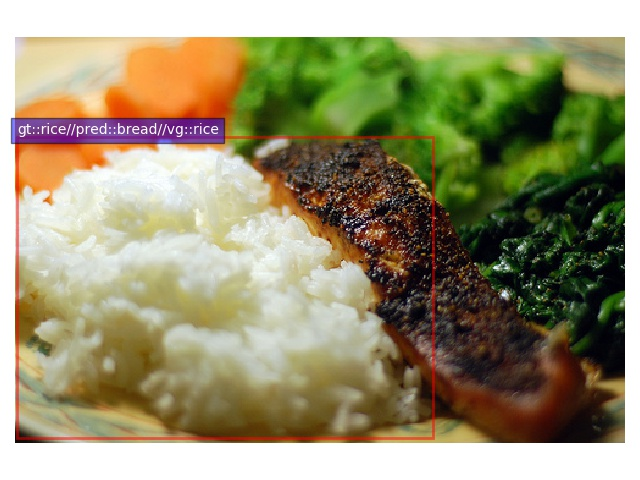
\includegraphics[scale=.2]{images/2323938.jpg}
	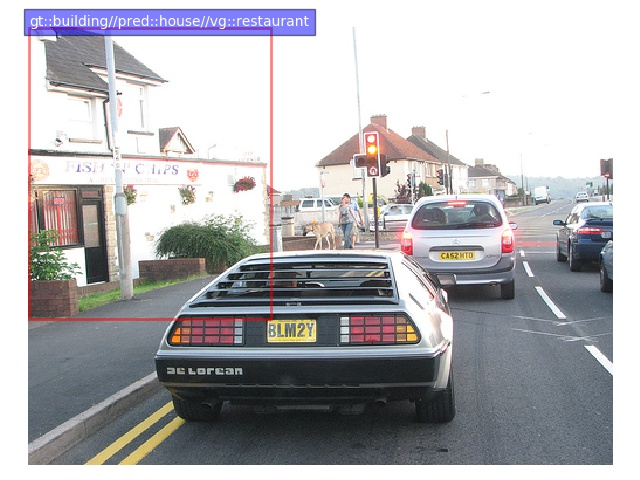
\includegraphics[scale=.2]{images/2322259.jpg}
	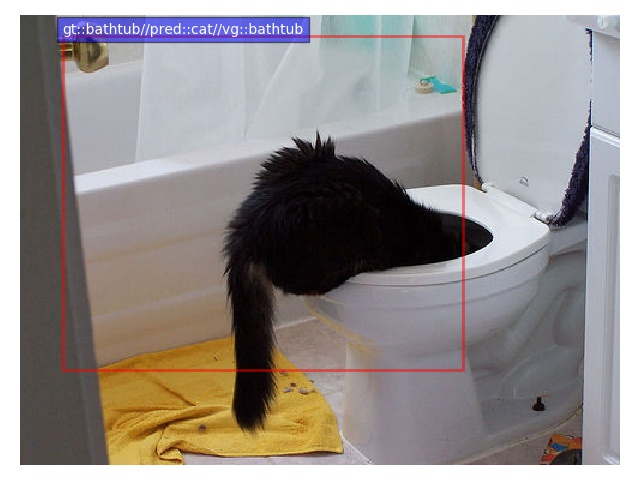
\includegraphics[scale=.2]{images/2371657.jpg}
	
	\caption{TODO: examples resnet mistakes (trained on vg\_manynames, tested on manynames-442)\label{fig:mistakes} \gbt{Will we have space for the figure? (Maybe we should \textit{make} space?) Also, shouldn't we put examples from the most successful model instead?}}
\end{figure}

\begin{figure}
	\centering
	\footnotesize
	\begin{tabular}{p{3.7cm}p{3.7cm}}
	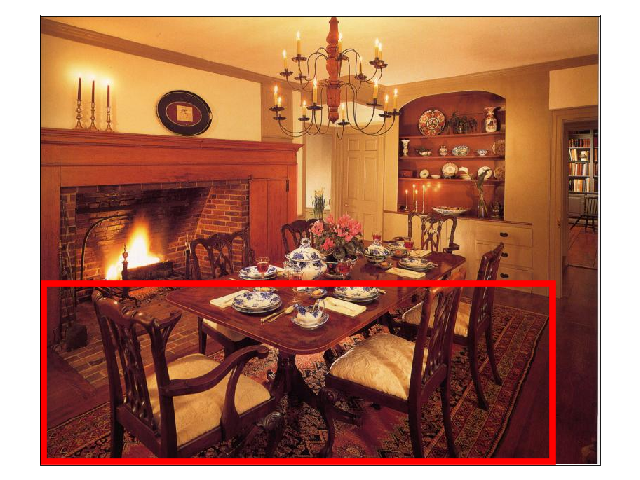
\includegraphics[scale=.2]{images/556_1063956_seed_ambiguous.png} &
	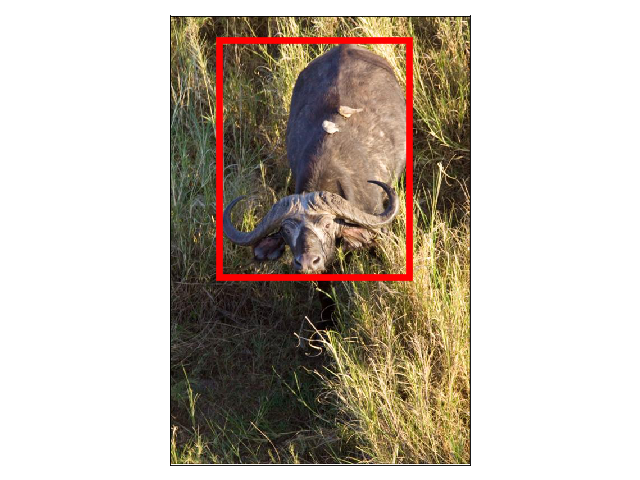
\includegraphics[scale=.2]{images/2657_1069343_singleton_obj.png} 
	\\
	Entry-level: rug (21) &  animal (9)\\
	\midrule
	Same-object: carpet (4, 0.7) &  yak (3,0.8), buffalo (2,0.7) \\
	Error-box: chair (5, 0.5), floor (3, 0.5) & \\
	Error-visual:  & cow (6,0.5), ram (3,0.7), bull (2,0.7)\\
	\midrule
	FRCNN$_{\text{VG1600}}$: floor & animal\\
	FRCNN$_{\text{VG1600--VGMN}}$: rug & cow \\
	\end{tabular}
	\caption{Annotations, verification and predictions for 2 objects: name (number of annotations, adequacy rating)}
\end{figure}

\subsection{How do predictions correlate with human agreement?}

An important observation in Section \ref{sec:manynames} is that even the high number of annotations for an object in ManyNames might not be enough to be fully confident about the entry-level name.
This suggests that there is a certain portion of objects in the dataset that could be difficult to name even for humans \sz{is it okay to claim this?}.
In Table \ref{tab:exp_errors_agreement}, we show the break-down of model predictions and errors for objects with high and low naming agreement in ManyNames, i.e.\ objects where more or less than 90\% of the annotators opted for the entry-level name. 
Here, we find a very clear pattern for all models, namely that the portion of hits is generally high when human agreement is also high.
Note that this even holds for the ResNet-based classifiers that generally achieve less accuracy.
When agreement is lower, all models produce less hits and more valid alternatives. 
This indicates that there is indeed a certain similarity between what is difficult for humans and models.
Interestingly, also the portion of incorrect predictions is substantially higher when the agreement is lower. \sz{why???}


%\cs{TODO::}
%Categorization of "errors" ():
%\begin{enumerate}
%	\item Clear mistake \\
%	e.g.,\ rice vs. bread
%	\item Alternative name\\
%	e.g.,\ building vs. house
%	\item Alternative object \cs{(other cluster from verif data)}
%	\item Synonym\\
%	e.g.,\ plane vs. airplane
%	\item Semantically related\\
%	e.g.,\  motorcycle vs. scooter
%\end{enumerate}










%%% Local Variables:
%%% mode: latex
%%% TeX-master: "acl2020_main"
%%% End:
